%%%%%%%%%%%%%%%%%%%%%%% file template.tex %%%%%%%%%%%%%%%%%%%%%%%%%
%
% This is a general template file for the LaTeX package SVJour3
% for Springer journals.          Springer Heidelberg 2010/09/16
%
% Copy it to a new file with a new name and use it as the basis
% for your article. Delete % signs as needed.
%
% This template includes a few options for different layouts and
% content for various journals. Please consult a previous issue of
% your journal as needed.
%
%%%%%%%%%%%%%%%%%%%%%%%%%%%%%%%%%%%%%%%%%%%%%%%%%%%%%%%%%%%%%%%%%%%
%
% First comes an example EPS file -- just ignore it and
% proceed on the \documentclass line
% your LaTeX will extract the file if required
\begin{filecontents*}{example.eps}
%!PS-Adobe-3.0 EPSF-3.0
%%BoundingBox: 19 19 221 221
%%CreationDate: Mon Sep 29 1997
%%Creator: programmed by hand (JK)
%%EndComments
gsave
newpath
  20 20 moveto
  20 220 lineto
  220 220 lineto
  220 20 lineto
closepath
2 setlinewidth
gsave
  .4 setgray fill
grestore
stroke
grestore
\end{filecontents*}
%
\RequirePackage{fix-cm}
%
%\documentclass{svjour3}                     % onecolumn (standard format)
%\documentclass[smallcondensed]{svjour3}     % onecolumn (ditto)
\documentclass[twocolumn,smallextended]{svjour3}       % onecolumn (second format)

\usepackage{multirow}
\usepackage{color}
\usepackage{dblfloatfix}
\usepackage{graphicx}
\usepackage{silence} \WarningFilter{fixltx2e}{}
\usepackage[cmex10]{amsmath}
\interdisplaylinepenalty=2500
\usepackage{amsfonts}

\usepackage[noadjust]{cite}
\usepackage[]{hyperref}
%\usepackage{cleveref}

\hypersetup{pdftitle={Urdu Handwritten Text Recognition},
colorlinks=true,citecolor=blue,linkcolor=red}

%\ifCLASSOPTIONcompsoc
%\usepackage[tight,normalsize,sf,SF]{subfigure}
%\else
%\usepackage[tight,footnotesize]{subfigure}
%\fi
%%%%%--------------------------------------------------------------------------------
%\newcommand{\abs}[1]{\left\vert #1 \right\vert}
%\newcommand{\norm}[1]{\left\Vert#1\right\Vert}
%\newtheorem{definition}{Definition}
%\newtheorem{theorem}{Theorem}
%\newtheorem{lemma}{Lemma}
%\newtheorem{proposition}{Proposition}[section]
%\newtheorem{remark}{Remark}

\newcommand*{\img}[1]{%
    \raisebox{-.02\baselineskip}{%
        \includegraphics[
        height=\baselineskip,
        width=\baselineskip,
        keepaspectratio,
        ]{#1}%
    }%
}

\newcommand*\inlinegraphics[1]{%
  \settototalheight\myheight{Xygp}%
  \settodepth\mydepth{Xygp}%
  \raisebox{-\mydepth}{\includegraphics[height=\myheight]{#1}}%
}
\makeatletter
\def\BState{\State\hskip-\ALG@thistlm}
\makeatother
%%%%--------------------------------------------------------------------------------

%%%%--------------------------------------------------------------------------------
\newcounter{MYtempeqncnt}    % Required for IEEE double column equations which unfortunately our paper has!!


%\ifCLASSINFOpdf
%  % \usepackage[pdftex]{graphicx}
%  % declare the path(s) where your graphic files are
%  % \graphicspath{{../pdf/}{../jpeg/}}
%  % and their extensions so you won't have to specify these with
%  % every instance of \includegraphics
%  % \DeclareGraphicsExtensions{.pdf,.jpeg,.png}
%\else
%  % or other class option (dvipsone, dvipdf, if not using dvips). graphicx
%  % will default to the driver specified in the system graphics.cfg if no
%  % driver is specified.
%  % \usepackage[dvips]{graphicx}
%  % declare the path(s) where your graphic files are
%  % \graphicspath{{../eps/}}
%  % and their extensions so you won't have to specify these with
%  % every instance of \includegraphics
%  % \DeclareGraphicsExtensions{.eps}
%\fi



\begin{document}
%
% paper title
% Titles are generally capitalized except for words such as a, an, and, as,
% at, but, by, for, in, nor, of, on, or, the, to and up, which are usually
% not capitalized unless they are the first or last word of the title.
% Linebreaks \\ can be used within to get better formatting a0s desired.
% Do not put math or special symbols in the title.
\title{Multi-Aspect Urdu Handwriting Data Collection}
%\title{A Survey on Urdu Handwritten Text Recognition: Tasks, approaches and applications}

%% author names and affiliations
%% use a multiple column layout for up to three different
%% affiliations
%\author{
%    \IEEEauthorblockN{
%		Mujtaba Husnain\IEEEauthorrefmark{1},
%		Malik Muhammad Saad Missen \IEEEauthorrefmark{1},
%		M. Abid Manzoor \IEEEauthorrefmark{1},\\
%		Micka\"{e}l Coustaty\IEEEauthorrefmark{2}, 
%		Muzzamil Luqman\IEEEauthorrefmark{2} and
%		Jean-Marc Ogier\IEEEauthorrefmark{2}}
%		\vspace{0.25cm}
%		
%    \IEEEauthorblockA{
%        \begin{tabular}{cc}
%            \begin{tabular}{@{}c@{}}
%                \IEEEauthorrefmark{1}
%					The Islamia University of Bahawalpur\\
%					, Pakistan\\
%					(mujtaba.husnain,saad.missen)@iub.edu.pk
%            \end{tabular} & \begin{tabular}{@{}c@{}}
%                \IEEEauthorrefmark{2}
%					L3i Lab, University of la Rochelle\\
%					Av. Michel Cr\'epeau, 17000 La Rochelle, France\\
%					(mickael.coustaty, mluqma01, jean-marc.ogier )@univ-lr.fr
%            \end{tabular}
%        \end{tabular}
%    }
%}
\author{Mujtaba Husnain$^1$,
		Malik Muhammad Saad Missen$^1$,
		M. Abid Manzoor$^1$,\\ \and 
		Mickaël Coustaty$^2$ \and 
		Muhammad Muzzamil Luqman$^2$ \and 
		Jean-Marc Ogier$^2$
}

\institute{$^1$The Islamia University of Bahawalpur, Pakistan (mujtaba.husnain,saad.missen)@iub.edu.pk\\
$^2$ L3i Lab, University of la Rochelle, Av. Michel Cr ́epeau, 17000 La Rochelle, France (mickael.coustaty, mluqma01, jean-marc.ogier )@univ-lr.fr}



\newcommand{\red}[1]{\textcolor{red}{#1}}


\date{Received: date / Accepted: date}
% The correct dates will be entered by the editor



% make the title area
\maketitle


\begin{abstract}
Work on the problem of handwritten text recognition in Urdu script has been an active research area and also a significant progress has been made in the last few years. In this paper a comprehensive overview is presented for various offline and online handwritten text recognition systems for Urdu script written in Nastaliq font style from year $2002$ to $2017$. Following features make our contribution worthwhile and unique among the reviews of similar kind: (i) our review classifies the existing studies on the basis of types of recognition systems used for Urdu handwritten text recognition (ii) it covers a very different outlook of the handwritten text recognition field by discussing the work at different granularity levels (like character, word, ligature, or sentence level) (iii) this state-of-art review also presents each of surveyed articles in following dimensions:  the designated task which it completed, its granularity level, dataset used, results obtained, and future dimensions, (iv) and lastly it gives the summary of the related articles according to the granularity levels, publishing years, related tasks or subtasks, and types of classifiers used. In the end, major challenges and tasks related to Urdu handwritten text recognition approaches are also discussed.
\end{abstract}



\section{Introduction}
Handwriting recognition is an active area of research in the field of pattern recognition and has various application in industrial and professional applications. Some of these applications include forms processing in government, administrative, health and academic institutes; postal address recognition, processing of bank cheques etc. Handwriting recognition concerns with automatic transforming a source language into its symbolic representation. The source language can be represented either in its spatial (offline) or temporal (online) \cite{61} form in graphical marks. In depth analysis of handwritten text give rise to a number of useful applications such as author profiling, named entity recognition, recognition of overlapped characters etc.\\
In late 1950\'s the first Optical Character Recognition (OCR) system was developed for the recognition of Latin text \cite{62, 63} which deals with recognition of numerals only. With the advancements in OCR, the systems available nowadays is expanded to recognize Latin script, and characters of a variety of other languages like Chinese, Japanese, Arabic, Persian etc.\\
Optical character recognition of Urdu script was started in late 2000 \cite{7} and the first work on Urdu OCR is published in 2004. The literature veview identified the fact that tnere has been lack of research efforts in Urdu handwritten text recognition as compared to recognition of other language scripts \cite{5, 7, 27}. There are few Urdu OCR systems for printed text that are commercially available \cite{64, 65} but there is no system available for Urdu handwritten text recognizing to date.\\
In verbal communication, Urdu language adopted many dialects across the regions but in formal writing Urdu script uses standard way. It is also observed that Urdu written script shares similarities with other languages like Arabic and Persian \cite{21}. Therefore, automatic interpretation of Urdu handwritten text would have prevalent and ubiquitous benefits.\\
Urdu handwriting is used for official assignments and communications in all the organizations in Pakistan. Most of the time, all this data (provided in the form of handwritten applications or forms) is typed into computers for further processing that requires a huge man power, processing equipment, time, money and other resources. For example data entry in NADRA offices for processing requests of National Identity Cards (NIC), student’s applications in government institutes, signature on banker cheques etc require an automatic Urdu handwritten text recognition tool to recognize the text and process the documentation in real time environment. Furthermore, the system should provide facility to save the information in some appropriate database. This will reduce a significant number of resources in daily official matters considering the nature of this task.\\
The development of Urdu handwritten recognition system can assist in reading historic Urdu manuscripts to make the content of these manuscripts available. The content of manuscripts is written in clear and readable way as compared to handwritten text which makes the task of recognition of contents of manuscript much simpler. On the other hand some issues associated with handwritten text make the task of developing the system for recognition of handwritten text more challenging and complicated. Some of these issues are differences in writing style (even from the same author), image degradation due to cursive nature of the script, poor quality or illegible handwriting etc.\\
This survey article gives a comprehensive survey of Urdu handwritten text recognition. Most recent survey articles on this topic were published in 2013 \cite{7, 66, 71}. As mentioned above, this survey article focus on the literature related to offline Urdu handwritten text recognition. Furthermore, some recent notable work can be found in \cite{67, 68, 69, 70} for recognition of printed Urdu text.\\
This paper is organized as follows: A brief introduction of Urdu script is given in~\ref{UrduSC}. In Section~\ref{ICR} we describe basic steps in ICR by describing the usual process of text recognition. Then in Section~\ref{sec:Review}, state-of-the art discussion on the existing work related to Urdu ICR script at different granularity levels is discussed in detail. Open issues, future directions and detailed analysis on the existing work is presented in Section~\ref{sec:DataAnalysis}. Section~\ref{Con} concludes the review.
\section{Urdu Script}\label{UrduSC}
Urdu is the national language of Pakistan and also considered as one of two official languages of Pakistan \cite{60} (with the other being English). It is widely spoken and understood as a second language by a majority of people of Pakistan \cite{1,2} and also being adopted increasingly as a first language by the people living in urban areas of Pakistan. //
Urdu script is written from right to left while digits are written from left to right, this is the reason Urdu can be considered as one of the bidirectional languages. Urdu script consists of 38 basic letters shown in Figure~\ref{fig1}. This alphabet set is also considered as superset of all Urdu script-based languages’ alphabets, i.e. Arabic contains 28 and Persian contains 32 \cite{4}. Furthermore, Urdu script also contains some additional alphabets to express the Hindi phonemes. Both Hindi and Urdu languages \cite{4} have same phonology with only difference in written script. All Urdu script-based languages such as Arabic and Persian have some unique characteristics i.e. (i) the script of these languages is written from right to left in cursive style and (ii) the script of these languages is context sensitive i.e. written in the form of ligatures which is a combination of a single or many alphabets. Due to this context sensitivity, most of the alphabets have different shapes depending on their position and their adjoining character in the word \cite{5}. This connectivity of alphabets \cite{6} has enriched the Urdu vocabulary with almost 24,000 ligatures. \\
%%%%%------- Figure 1 --------------------------------------------------------------------------------------
\begin{figure}
\centering
	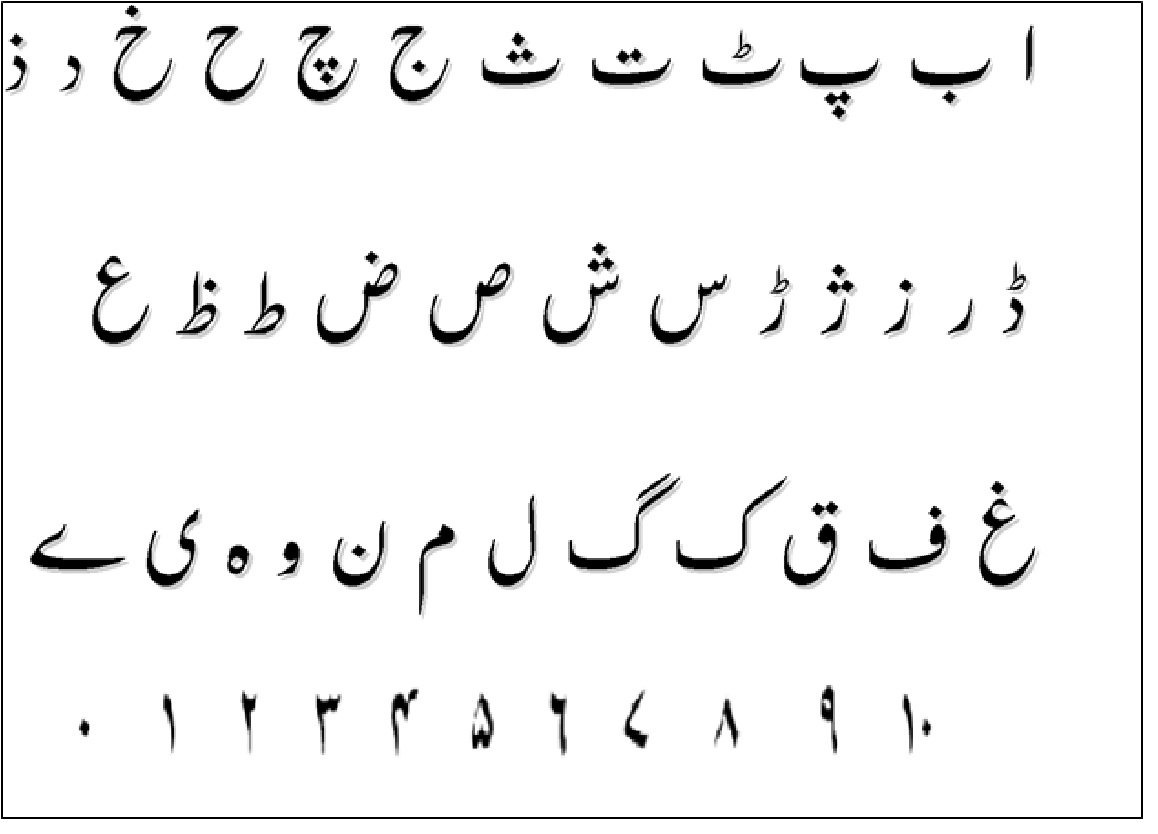
\includegraphics[width=8.cm]{Urdu_alphabets.jpg}
\caption{Basic alphabets and numerals of Urdu script}\label{fig1}
\end{figure}
%%%%%------- Figure 1 --------------------------------------------------------------------------------------
In Urdu script, alphabets are classified in two groups: joiner and non-joiner. The joiner characters join to other characters on initial, middle and end position in the ligature. While non-joiner appear in isolated form. Figure~\ref{fig2} shows list of joiner and non-joiner alphabets of Urdu script. While writing Urdu script one can write the words in which letters overlap each other without touching. This overlapping make the segmentation of words to characters more complex and challenging while using segmentation-based approach.\\
Naskh and Nastaliq are two widely used fonts in which Urdu script is written. Nastaliq is more complex than Naskh as Nastaliq \cite{4} has variety of variations of shape of an alphabet depending on its position in the word as compared to Naskh e.g. the second alphabet \img{Bay.png}(bay) has different shapes while appearing in any position in a word shown in Figure~\ref{fig2}.\\ 
%%%%%------- Figure 2 --------------------------------------------------------------------------------------
\begin{figure}[t]
\centering
	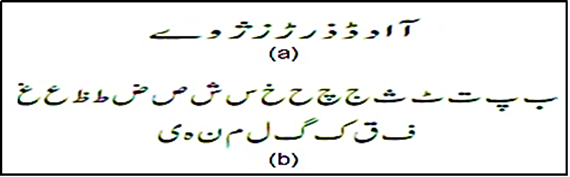
\includegraphics[width=8.cm]{joiner.png}
\caption{(a) Non joiner and (b) Joiner alphabets in Urdu script}\label{fig2}
\end{figure}
%%%%%------- Figure 2 --------------------------------------------------------------------------------------
Above mentioned issues make the recognition of Urdu handwritten text more challenging as compared to any other script. There are some inherent characteristic features of Urdu script that may enable the recognition process of Urdu handwritten text. These features include accent and diacritical marks that help in differentiating  one character from the other, different shapes of same letter based on its position in the word, presence of the virtual line (baseline). 
It is also mentioned by a number of researchers that reason behind the assumption that recognition of Urdu handwritten text is more difficult is absence of the appropriate resources and required techniques.\\
\section{Intelligent Character Recognition (ICR)} \label{ICR}
In the field of computer vision and pattern recognition, intelligent character recognition (ICR) is the process of recognition of handwritten text that is given as input to a computer.  The process of handwriting recognition primarily depends on optical character recognition (OCR). However, a complete handwriting recognition system also includes correct segmentation of words into characters, formatting of the extracted segment and finding the most reasonable words. For rest of paper the term ICR will be used for handwritten text recognition. There are some issues in ICR such as  change in font, slope of line, different writing style even from single writer, overlapping joining letters, missing placement of dots and diacritics aka secondary strokes etc that make process of ICR more challenging than the recognition of printed text. These issues become more complicated in Urdu ICR because of its cursive script in which character changes its shape based on its position in a word \cite{3}. These issues are discusses in detail in subsequent subsections below. \\
\subsection{Urdu based ICR systems}
Urdu based ICR systems can be divided into two types i.e. Online and Offline. In Online ICR, real time recognition of characters is performed using sensors to detect and analyze the pen tip movement, stroke position, baseline detection etc. While in Offline, character recognition implicates the automatic conversion of handwritten text from scanned image of paper. Offline character recognition is a complex process than online character recognition\cite{8,9,10}. \\
In practice, the text data is given as input in the form of scanned image that is analyzed and recognized as machine readable characters. The text data may have different fonts and handwriting styles that needs to be preprocessed to produce an ideal and clear view of the input data. ICR is different from OCR in a sense that ICR is associated with handwritten text recognition while OCR works on recognition of printed text. A typical ICR system comprised of three phases: (i) preprocessing, (ii) segmentation and (iii) recognition.\\ 
In first phase, a set of operations are performed in order to reduce the ink-noise ratio because the input set of handwritten documents may include inconsistent text due to having different writing styles. These operations include skewness smoothing, chain coding and baseline removal \cite{5, 7}. In segementation phase, the scanned image is segmented at three levels mentioned in \cite{8,9}. In order to get the finer results from segmentation, one must have to move through all the three levels. In last phase, recognition is performed in which the segmented text data is scanned and matched with the stored training set data.\\ 
The application of ICR has increased its efficacy towards automatic recognition of real world handwritten documents to make them useful for various business and academic applications.

\subsection{Contribution}
In this paper, our contribution revolves around following objectives:
\begin{itemize}
\item To provide a multi-aspectual dataset to the researchers for Urdu ICR development, this will save a lot of time and effort of the research team,
\item To collect data from individuals of various fields, age, gender and disorders for development of a mature and large variety of styles in Urdu script dataset,
\item To include handwriting of handicaps, partially blind, primary level students, calligraphers and individuals while traveling.
\item To provide an annotated data collection for researchers working for Urdu processing technologies, 


\end{itemize}

\section{Existing Urdu Data Collections}
\label{sec:Review}

Some Offline Urdu handwritten databases available are CALAM, UPTI, UCOM or UNDH and CENPARMI. Only UNHD is available freely while other data collections access is not free. 
The concept of creating Urdu handwritten dataset was first conceived in 2013 at computer science department of COMSATS Institute of Information Technology (CIIT) Abbottabad. Firstly, data was collected from 100 students on 6 papers having 8 text lines on each paper. Base lines were removed and text line segmentation was performed on collected data \cite{ahmedsb}. This Urdu dataset was collected at CIIT. With this affiliation we named it as UCOM dataset. UCOM was published in 2015. \\
The extension of UCOM dataset is UNHD which is an abbreviation of ‘Urdu Nastaliq Handwritten Dataset’. In these Urdu handwritten samples gathered from school students, college graduates, and office going individuals.  In this text for dataset broadened from 48 lines to 700 unique text lines. These lines included Urdu numeric and Urdu constraint handwritten samples. \\
CENPARMI \cite{sagheer} is considered to be the first handwritten-Corpus for Urdu language. This consists of digits and characters of Urdu-script. It is a huge database for Urdu-handwritten texts. It contains 57 Urdu-words, 44 isolated-characters, dates in different formats, isolated-digits, numeric strings with and without-decimal points, and 5 special-symbols. It formed the world’s first database for offline Urdu handwritten recognition; which was designed at Centre for Pattern-Recognition and Machine-Intelligence (CENPARMI).\\
Urdu Printed-Text Image (UPTI) is a dataset that was developed for research-community as an analogy to-APTI dataset. This consists of different adaptation to-measure accuracy of the recognition-system for Urdu Language. These adaptations consist of ligatures or sub words, degraded-text-lines and degraded-ligatures. The text lines included were selected-from Jang newspapers. These lines include different topics of politics, religion and social-issues. This dataset consists of 10000 images with having Urdu text lines and 970649 characters \cite{naz2010}.\\
CALAM provides us a way for healing and fetching of information in a scientific and systematic-aspect. This uses design and development of an annotated-corpus of handwritten text-image \cite{ch2015}. This is a suitable mechanism to-annotate linguist handwritten-image dataset. Away from pure text-glossary, CALAM contribute some additional linguistics features-about the nature of language such as-document of corpus to-other language. CALAM-provides us a terrace for linguist Corpus-convenient for all types of linguistic-linked to research, where a large-scale of fine grade systematic-data crosswise language is maintained in both handwritten-and machine-readable format.

%%%%%------- Table 6 --------------------------------------------------------------------------------------
\begin{table*}[t]
\centering
\caption{Details of Urdu datasets}\label{tab6}
\begin{tabular}{@{}lll@{}}
\hline
Dataset	& Statistics & Price \\ \hline
& Total number of writers 500 & Public\\
& Text lines per page 8 & \\
UNHD \cite{15} & Total number of text lines 10,000 &\\
& Total Number of words 312, 000 &\\
& Total number of characters 187, 200 &\\ 
 \hline
& Total number of writers 250 & US\$250\\
UPTI\cite{21} & Total number of text images 10,000 \\
& Text lines per page 6 \\
& Total number of characters 9, 70, 650 &\\
\hline
& Total number of writers 343 & US\$500 \\
CENPARMI \cite{32} & Total number of text images 19,432 &  \\
& Total samples of Urdu handwritten digits 180 &\\
\hline
& Total number of writers 725 & US\$400\\
& Total number of images 1,200 &\\
CALAM \cite{58} & Total number of text lines 3,043  &\\
& Total number of words 46, 664 &\\
& Total number of ligatures 101,181 &\\
\hline
 \end{tabular}
\end{table*}
%%%%%------- Table 6 --------------------------------------------------------------------------------------


\section{Multi-Aspect Urdu Handwritten Data Collection}
The proposed data collection is unique in its approach towards building an annotated data collection for Urdu handwriting recognition. We propose this data collection with focus on those authors that are likely to have very unique writing styles because of their professions or because of some disabilities. Currently, there exists no data collection which involves such variety of authors. Another uniqueness of proposed data collection lies in use of same text for all authors. This opens ways for research in author attribution and graphology tasks in Urdu handwriting. We make this data collection freely available for research purposes which is another positive feature of proposed data collection. 

Preparing this data collection involves following steps:
\begin{itemize}
\item Selecting participants for writing,
\item Selecting Content for Writing,
\item Preparing Annotation forms and Annotation Guidelines
\item Annotating Dataset

\end{itemize}

\subsection{Participants Selection}

This step makes our data collection unique because we have chosen a variety of participants not only with different demographics but with the likelihood of producing different styles of Urdu handwriting. In this subsection, we provide details of all categories of selected participants along with images of their written samples. 
\subsubsection{Students}
Firstly we have included the student’s category, which is further divided into three sub-categories.
First of them is Primary level students. In which students of both gender male/female are included with age group of b/w 10-12 years. We have 5 male students and 5 female students. We also want to include left hand writer but unfortunately we did not have any one among these 10.
%%%%%------- Figure 3.2 --------------------------------------------------------------------------------------

%%%%%------- Figure 2 --------------------------------------------------------------------------------------

Second sub-category of students was Matric level students. In which students of both gender male/female are included with age group of b/w 13-16 years. We have 5 male students and 5 female students. We also want to include left hand writer in this category, we only found 2 students among these 10.
%%%%%------- Figure 3.3 --------------------------------------------------------------------------------------

%%%%%------- Figure 2 --------------------------------------------------------------------------------------
Third sub-category of students was Graduate level students. In which students of both gender male/female are included with age group between 20-30 years. We have 7 male students and 8 female students. We also want to include left hand writer in this category, but unfortunately we did not have any one among these 15.

%%%%%------- Figure 3.4 --------------------------------------------------------------------------------------


Please see figures \ref{fig3_2},\ref{fig3_3},\ref{fig3_4},\ref{fig3_5},\ref{fig3_6},\ref{fig3_7} in appendix for writings of students category. 

\subsubsection{Doctors}
Second is the doctor’s category. It includes doctors of both gender male/female. We have 5 male and 5 female doctors. We also want to include left hand writer but unfortunately we did not have any one among these 10.
%%%%%------- Figure 3.8 --------------------------------------------------------------------------------------

%%%%%------- Figure 2 --------------------------------------------------------------------------------------

Please see figures \ref{fig3_8} and \ref{fig3_9} in appendix for writings of doctors category. 
\subsubsection{Office Clerks}
The third category is of official clerks. It includes 4 male and 1 female clerks. All 5 clerks are right-handed.

%%%%%------- Figure 3.10 --------------------------------------------------------------------------------------

%%%%%------- Figure 2 --------------------------------------------------------------------------------------

%%%%%------- Figure 3.11 --------------------------------------------------------------------------------------

%%%%%------- Figure 2 --------------------------------------------------------------------------------------
Please see figures \ref{fig3_10} and \ref{fig3_11} in appendix for writings of office clerks category. 
\subsubsection{Land Record Officials}

The fourth category includes land record officials. It includes only male officials. All are right-handed.

%%%%%------- Figure 2 --------------------------------------------------------------------------------------
Please see figure \ref{fig3_12} in appendix for writings of land record officials category.
\subsubsection{Travelers}
Fifth category is of travelers. It includes both gender male/female with age group b/w 25-30 years. We have 1 male and 1 female writer. Both are right-handed.

Please see figures \ref{fig3_13} and \ref{fig3_14} in appendix for writings of travelers category.
%%%%%------- Figure 2 --------------------------------------------------------------------------------------


\subsubsection{Stamp Papers Seller}
It is the sixth category. It includes only males and all are right-handed. Unfortunately we couldn’t find any left-handed seller.
%%%%%------- Figure 3.15 --------------------------------------------------------------------------------------

%%%%%------- Figure 2 --------------------------------------------------------------------------------------
 Please see figures \ref{fig3_15} in appendix for writings of stamp seller category.
\subsubsection{Old Educated}
The seventh category is of old educated people. It includes both gender male/female. There are 6 males and 4 female writers. All writers are right-handed.
Please see figures \ref{fig3_16} and \ref{fig3_17} in appendix for writings of old age educators category.

\subsubsection{Special Persons}

\paragraph{Partially Blind}: The last one is special person’s category, which is further divided into three sub-categories.First of them is 'partially blind’. It includes both gender male/female with age group b/w 15-20 years. We have 4 male individuals and 1 female.  Among the 5, one is left-handed writer and 4 are right-handed. Please see figures \ref{fig3_18} and \ref{fig3_19} in appendix for writings of special persons category.
%%%%%------- Figure 3.18 --------------------------------------------------------------------------------------

%%%%%------- Figure 2 -------------------------------------------------------------------------------------

\paragraph{Physically Disabled}: Second of them is physically issues. It includes 3 male writers.  2 are left-handed writer and 1 is right-handed. Please see figures \ref{fig3_20} and \ref{fig3_21} in appendix for writings of physically disabled category.




\paragraph{Ambidextrous}:The third one is Ambidextrous. It describes individuals who can use either hand to write. It includes two female writers of age group between 18 to 27. Please see figures \ref{fig3_22} and \ref{fig3_23} in appendix for writings of Ambidextrous category.


%%%%%------- Figure 3.22 --------------------------------------------------------------------------------------


\subsection{Selecting Content for Writing }

\subsection{Preparing Annotation Forms and Annotation Guidelines }
For the collection of data set, we have invited 84 individuals from different categories. Each individual was asked to write the set of 10 A4 size pages. Each individual was directed to write the printed text in his/her in black. They were also given directions to how to write on the pages. Furthermore, they were also asked to provide the some personal information like name, age, gender, disease (if any), category (right/left hand writer, profession like student, doctor, etc). A sample of this information is depicted in the figure~\ref{fig3_1} below (it is not made public with data collection, it is only an example).

%%%%%------- Figure 3.23 --------------------------------------------------------------------------------------
\begin{figure}[t]
\centering
	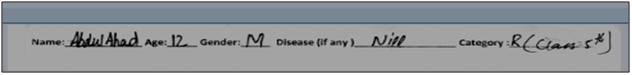
\includegraphics[width=8.cm]{figures/Fig3_1.png}
\caption{Header of the Annotation Form}\label{fig3_1}
\end{figure}
%%%%%------- Figure 2 -------------------------------------------------------------------------------------

All the writers are directed to follow our instructions. Some of the individuals also draw baseline using lead pencil for their convenience while writing.  Some of the officers and students wrote in blue because writing in blue is more common than in black.



\subsection{Annotating Data Set }

Aletheia is a leading system for scientific use and still cost effective. It is used for recognition and annotation of scanned documents. Its main function is to create and to view page partition and OCR ground truth. Storage format of page is XML. Third party software supported page is also viewed by this. We are using Aletheia version 3(pro), which is latest version in market. Listed below are some page features of Aletheia:

\begin{itemize}
\item Page elements on four levels regions, text lines, words and glyphs
\item Remove noise from selected element by smearing option
\item Add annotation/ text of selected element
\item Change color document into black and white image.
\item Document border
\item Metadata
\item Page collections
\end{itemize}





\section{Data Analysis}
\label{sec:DataAnalysis}
\subsection{Data Set Details}

Table \ref{tabdataset} describes a summarized review of our data collection in comparison with existing Urdu data collections. The proposed data collection stands unique as far as variety of different styles is concerned contributing significant number of words.  

\begin{table}[t]
\centering
\caption{Comparison of Existing Datasets with Our Dataset}\label{tabdataset}
\begin{tabular}{|p{1.2cm}|p{0.6cm}|p{0.6cm}|p{1.5cm}|p{0.5cm}|p{0.7cm}|p{0.5cm}|}
\hline
\begin{flushleft}
\textbf{Details	}
\end{flushleft}& \begin{flushleft}
\textbf{UCOM}
\end{flushleft} & \begin{flushleft}
\textbf{UNHD}
\end{flushleft} & \begin{flushleft}
\textbf{CENPARMI}
\end{flushleft} & \begin{flushleft}
\textbf{UPTI}	
\end{flushleft}& \begin{flushleft}
\textbf{CALAM}
\end{flushleft} &	\begin{flushleft}
\textbf{Our Data Set}
\end{flushleft} \\ \hline
Approx. no of words per-page &	104	& - & - & - &	-&	130 \\ \hline
No. of text lines per-page	& 8	& 5 to 8 & - & - &	3 to 5	& 8 to 12 \\ \hline
No. of pages per writer	&6&	6&	2& - & -&			10 \\ \hline
Approx. no. of words per writer &	620	& 624& -&-&-&				1381 \\ \hline
Total number of words	& 62000	&312000	&20 digits, freestyle date, 38 numeral stings, 43 characters, 57 words, 5 special symbols		& -& 46664	& 114623 \\ \hline
Total number of lines &	6400 &	10,000&-&		10063	&3043&	9379 \\ \hline

Total number of pages&	600	&3000&	686	&-&	1200&	830 \\ \hline

Number of writers	& 100&	500	&343&-&		725&	83 \\ \hline

Categories&	Only students&	Students and Professionals &	3(left handed/ right handed)&	Text consisted of different-social, religious and political issues	&6 (subject based)&	8 \\ \hline
Special persons writing	& - & - & - & - & - &			10 \\ \hline

Publicly available	& Yes	&yes&	No&	No&	No&	Yes \\ \hline


\hline
 \end{tabular}
\end{table}
%%-------------------------------

In the following subsections, we analyze writing patterns of different set of authors for different aspects. Handwriting Analysis is described as a scientific study and analysis of handwriting. It is a way of interpreting behavior from peculiarities in handwriting. The scientific name for handwriting analysis is Graphology \cite{graphology}. It helps in determining the psychological behavior and profession of the authors. Unfortunately, we lack psychological theories for Urdu handwriting styles; however, we plan to compare lengths and width of different words because size of the word does matter in graphology. 


\subsection{Comparing Length and Width of Words over Categories}

In this subsection, we compare length and width of a selected set of words over different categories. Words are selected according to their length i.e. words are chosen from a category of words of length two, three, four, five, six and seven. The idea behind this interesting task is to seek if a particular category of authors can be found using a particular style for a set of words. Figures \ref{figclerks}, \ref{figdoc}, \ref{figlo}, \ref{figoed}, \ref{figsp}, \ref{figstd}, \ref{figstamp}, \ref{figstrav}, \ref{fig:sfig9} and \ref{fig:sfig10} represent graphs for various categories. All graphs do not reveal something very big but there are some interesting observations that can be made. For example, it is evident from the graphs that as the width of a word increases (with more number of alphabets), its height also increases. Normally, width and height of a word are not co-related but in this particular scenario it is understood because as the width of a word increases it involves various types of alphabets involving accents which cause an increase in height too. The first four words mentioned on x-axis start around 60 pixels in height and width for all categories. Average of 5th, 6th and 7th words remains around 80 while last two words get peaks because of their increased length and height. There is nothing extra ordinary that can be mentioned as far as cross-category examination is concerned. 









%%% -------------------- table of pictures 
% \begin{table}[p]
%     \begin{center}
%     \begin{tabular}{  c  p{5cm} }
     
      
 %    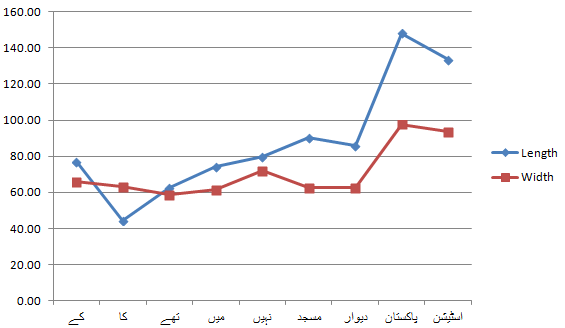
\includegraphics[width=0.4\textwidth, height=40mm]{graphs/clerks.png}
%      & 
 %    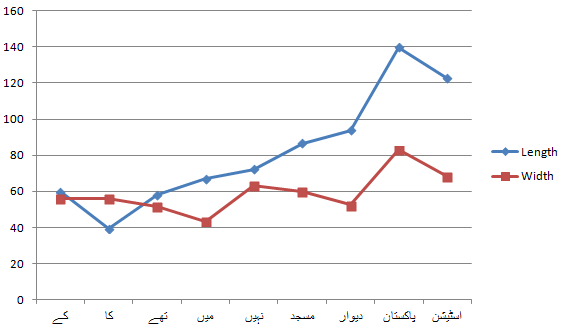
\includegraphics[width=0.4\textwidth, height=40mm]{graphs/doctors.png}
      
%      \\ 
%      \end{tabular}
%      \caption{Word Length Analysis as written by different categories of authors}
%      \label{tbl:myLboro}
%      \end{center}
%      \end{table}
      
%%%%% --------------------------------------------------------------


 




\subsection{Comparison for the size of words according to its position in script}

In this subsection, we analyze if position of a word affects its width while writing. This analysis is performed over all categories of authors by selecting a set of words of different lengths. Figures \ref{fig:sfig11}, \ref{fig:sfig12}, \ref{fig:sfig13}, \ref{fig:sfig14}, \ref{fig:sfig15} show width of different words with respect to their positions written by different authors of different categories. The idea behind this analysis is to see if authors squeeze their words when they have a limited space problem. A detailed observation of these graphs shows that most of the writers write freely when in start of a line while they squeeze their words when approaching end of the line. It can be important feature to be considered when working on handwriting recognition. 







\subsection{Analyzing Different Patterns of a Letter According to Category of Authors}

Tables \ref{tab6-student},\ref{tab6-ssc},\ref{tab6-pdp},\ref{tab6-lro},\ref{tab6-trav},\ref{tab6-doc},\ref{tab6-led} highlight different styles used by a particular category of authors for a specific Urdu alphabet. Looking at various patterns present in different tables for all alphabets, it can be concluded that highest variance in writing styles can be observed in Patwaris (see table \ref{tab6-lro}) and Stamp Sellers (see table \ref{tab6-ssc}) category while others do differ in their style but more or less show similar patterns. 

\section{Conclusion} \label{Con}
Urdu script is categorized as one of the cursive and bidirectional script derived from Arabic this is the reason it shares almost similar challenges and issues but with higher complexity. In this paper, we propose a multi-aspectual Urdu handwriting data collection. We also give a review of existing data collections for Urdu handwriting recognition and give a comparison of the proposed data collection with existing ones. The uniqueness of the proposed data collection lies in the variety of authors known especially for their typical handwriting. Making same text written by all authors also make this data collection suitable for research tasks like author attribution and graphology. The proposed data collection will be made freely available for research purposes.  


%%%%%------- Table 6 --------------------------------------------------------------------------------------
\begin{table}[h]
\centering
\caption{Letter styles used by less educated persons}\label{tab6-led}
\begin{tabular}{@{}cccc@{}}
\hline
Letters	& \multicolumn{3}{c}{\textbf{Used Styles}} \\ \hline

\includegraphics[scale=0.50]{Alif.png} series & 
\includegraphics[scale=0.25]{alif_madd.PNG} & 
\includegraphics[scale=0.25]{ali_madd2.PNG}  & 
\includegraphics[scale=0.45]{alif_1.PNG}  \\ 
\hline

\includegraphics[scale=0.50]{Bay.png} series & 
\includegraphics[scale=0.20]{tai.PNG} & 
\includegraphics[scale=0.20]{tai2.PNG}  & 
\includegraphics[scale=0.20]{Tai3.png} \\
\hline

\includegraphics[scale=0.25]{jeeem} series & 
\includegraphics[scale=0.25]{chay} & 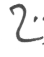
\includegraphics[scale=0.20]{jeem}  & 
\includegraphics[scale=0.15]{jeeem2} \\
\hline

\includegraphics[scale=0.25]{daal_orig.png} series & 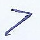
\includegraphics[scale=0.15]{Daal_2.png} & 
\includegraphics[scale=0.15]{Daal_3.png}  & 
\includegraphics[scale=0.15]{Daal_4.png} \\
\hline

\includegraphics[scale=0.25]{re_orig.png} series & 
\includegraphics[scale=0.15]{raay.PNG} & 
\includegraphics[scale=0.15]{raay2.PNG}  & 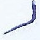
\includegraphics[scale=0.15]{re_1.png} \\
\hline

\includegraphics[scale=0.25]{seen_orig.png} series & 
\includegraphics[scale=0.15]{seen.PNG} & 
\includegraphics[scale=0.15]{seen2.PNG}  &  \\
\hline
\includegraphics[scale=0.20]{suad_orig.png} series & 
\includegraphics[scale=0.15]{zuwad2.PNG} & 
\includegraphics[scale=0.15]{Suad_4.png}  &  \\
\hline
\includegraphics[scale=0.15]{aien_orig.png} series & 
\includegraphics[scale=0.15]{aein.PNG} & 
\includegraphics[scale=0.10]{aein2.PNG}  &  \\
\hline
\includegraphics[scale=0.15]{tuay_orig.png} series & 
\includegraphics[scale=0.15]{tuin.PNG} & 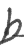
\includegraphics[scale=0.15]{tuin2.PNG}  & 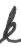
\includegraphics[scale=0.15]{zuin.PNG} \\
\hline
\includegraphics[scale=0.25]{fay_orig} series & 
\includegraphics[scale=0.25]{faay} & 
\includegraphics[scale=0.25]{23}  &  \\
\hline

\includegraphics[scale=0.20]{qaaf_orig} series & 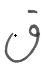
\includegraphics[scale=0.15]{kahf} & & \\
\hline
\includegraphics[scale=0.15]{kaaf_orig} series & 
\includegraphics[scale=0.15]{kaaf2} & 
\includegraphics[scale=0.15]{kaaf3}  & 

\includegraphics[scale=0.15]{kaaf} \\
\hline

\includegraphics[scale=0.15]{Laam_orig} series & \includegraphics[scale=0.15]{laaam} & \includegraphics[scale=0.15]{laam2}  &  \\
\hline
\includegraphics[scale=0.15]{meem_orig} series & \includegraphics[scale=0.15]{meem} & \includegraphics[scale=0.15]{meem2}  &  \\
\hline
\includegraphics[scale=0.15]{noon_orig} series & \includegraphics[scale=0.15]{noon_guna} & \includegraphics[scale=0.15]{noon} & 
\includegraphics[scale=0.15]{noon2} \\
\hline
\includegraphics[scale=0.15]{wao_orig} series & \includegraphics[scale=0.15]{capture} & \includegraphics[scale=0.15]{wao}  & 
\includegraphics[scale=0.15]{haaa} \\
\hline
\includegraphics[scale=0.15]{choti_ye_orig} series & \includegraphics[scale=0.15]{choti_yaa2} & \includegraphics[scale=0.15]{Bari_yaa2} & 
\includegraphics[scale=0.15]{bari_yaa} \\

 \end{tabular}
\end{table}
%%%%%------- Table 6 --------------------------------------------------------------------------------------


%%%%%------- Table 7 --------------------------------------------------------------------------------------
\begin{table}[h]
\centering
\caption{Letter styles used by Doctors}\label{tab6-doc}
\begin{tabular}{@{}ccccc@{}}
\hline
Letters	& Letters Family & \multicolumn{3}{c}{\textbf{Used Styles}} \\ \hline
\includegraphics[scale=0.35]{alif.png} series & \includegraphics[scale=0.35]{alif.png} \includegraphics[scale=0.20]{alif_mad_orig.png} & \includegraphics[scale=0.25]{1.png} &
\includegraphics[scale=0.25]{2.png} &
\includegraphics[scale=0.25]{3.png} \\ 
\hline
\includegraphics[scale=0.35]{Bay.png} series & \includegraphics[scale=0.45]{Bay.png} \includegraphics[scale=0.25]{pay.png}... & \includegraphics[scale=0.20]{4} &
\includegraphics[scale=0.15]{5} &
\includegraphics[scale=0.15]{6} \\ 
\hline
\includegraphics[scale=0.25]{jeeem} series & \includegraphics[scale=0.25]{jeeem} \includegraphics[scale=0.25]{chay_orig}... & \includegraphics[scale=0.20]{7} &
\includegraphics[scale=0.15]{8} &  \\ 
\hline
\includegraphics[scale=0.25]{daal_orig} series & \includegraphics[scale=0.25]{daal_orig} \includegraphics[scale=0.25]{dal} & \includegraphics[scale=0.20]{9} &
\includegraphics[scale=0.25]{10} & \\ 
\hline
\includegraphics[scale=0.25]{re_orig} series & \includegraphics[scale=0.25]{re_orig} \includegraphics[scale=0.25]{R'e}... & \includegraphics[scale=0.20]{11} &
\includegraphics[scale=0.15]{12} &  \\ 
\hline
\includegraphics[scale=0.25]{seen_orig} series & \includegraphics[scale=0.25]{seen_orig} \includegraphics[scale=0.25]{sheen} & \includegraphics[scale=0.25]{13} &
\includegraphics[scale=0.25]{14} & \\ 
\hline
\includegraphics[scale=0.25]{Suad_orig} series & \includegraphics[scale=0.25]{Suad_orig} \includegraphics[scale=0.25]{zuad} & \includegraphics[scale=0.25]{15} &
\includegraphics[scale=0.25]{16} & \\ 
\hline
\includegraphics[scale=0.25]{Aien_orig} series & \includegraphics[scale=0.25]{Aien_orig} \includegraphics[scale=0.25]{ghen} & \includegraphics[scale=0.25]{17} &
\includegraphics[scale=0.20]{18} & \\ 
\hline
\includegraphics[scale=0.25]{tuay_orig} series & \includegraphics[scale=0.25]{tuay_orig} \includegraphics[scale=0.25]{zuay} & \includegraphics[scale=0.25]{tuin} &
\includegraphics[scale=0.20]{tuin2} & 
\includegraphics[scale=0.20]{zuin}\\ 
\hline
\includegraphics[scale=0.20]{Fay_orig} series & \includegraphics[scale=0.20]{Fay_orig} & \includegraphics[scale=0.25]{22} &
\includegraphics[scale=0.20]{23} & \\ 
\hline
\includegraphics[scale=0.25]{qaaf_orig} series & \includegraphics[scale=0.25]{qaaf_orig} & \includegraphics[scale=0.20]{24} &
\includegraphics[scale=0.20]{25} & \\ 
\hline
\includegraphics[scale=0.20]{Kaaf_orig} series & \includegraphics[scale=0.20]{Kaaf_orig} \includegraphics[scale=0.20]{Gaaf_orig} &\includegraphics[scale=0.20]{26} &
\includegraphics[scale=0.20]{27} & \\ 
\hline
\includegraphics[scale=0.20]{laam_orig} series & \includegraphics[scale=0.25]{laam_orig} & \includegraphics[scale=0.25]{laam2} &
\includegraphics[scale=0.20]{28} & \\ 
\hline
\includegraphics[scale=0.20]{Meem_orig} series & \includegraphics[scale=0.20]{Meem_orig} & \includegraphics[scale=0.20]{30} &
\includegraphics[scale=0.15]{31} &  
\includegraphics[scale=0.20                                                                                                                                                                                                                                                                                                                                   ]{32}  \\
\hline
\includegraphics[scale=0.20]{noon_orig} series & \includegraphics[scale=0.25]{noon_orig} 
\includegraphics[scale=0.25]{noon_ghunna} & \includegraphics[scale=0.25]{33} &
\includegraphics[scale=0.20]{34} &  
\includegraphics[scale=0.20]{35}  \\
\hline
\includegraphics[scale=0.20]{wao_orig} series & \includegraphics[scale=0.25]{wao_orig}
\includegraphics[scale= 0.15]{haey_orig}
\includegraphics[scale=0.35]{hamza} & \includegraphics[scale=0.25]{36} & &  \\
\hline
\includegraphics[scale=0.15]{choti_ye_orig} series & \includegraphics[scale=0.15]{choti_ye_orig} \includegraphics[scale=0.20]{bari_ye} &\includegraphics[scale=0.20]{37} &
\includegraphics[scale=0.20]{38} & 
\includegraphics[scale=0.20]{39} \\ 
\hline
\end{tabular}
\end{table}
%%%%%------- Table 7 --------------------------------------------------------------------------------------

%%%%%------- Table 8 --------------------------------------------------------------------------------------
\begin{table}[h]
\centering
\caption{Letter styles used by Travellers}\label{tab6-trav}
\begin{tabular}{@{}ccccc@{}}
\hline
Letters	& \multicolumn{4}{c}{\textbf{Used Styles}} \\ \hline
\includegraphics[scale=0.50]{alif.png} series & \includegraphics[scale=0.20]{40} & \includegraphics[scale=0.20]{41}  & \includegraphics[scale=0.35]{42}  & \\ 
\hline
\includegraphics[scale=0.50]{bay} series & \includegraphics[scale=0.20]{43} & \includegraphics[scale=0.20]{44}  & \includegraphics[scale=0.20]{45} & \\
\hline
\includegraphics[scale=0.25]{jeeem} series & \includegraphics[scale=0.20]{46} & \includegraphics[scale=0.15]{47}  & \includegraphics[scale=0.15]{48} &
\includegraphics[scale=0.15]{49} \\
\hline
\includegraphics[scale=0.25]{daal_orig} series & \includegraphics[scale=0.15]{50} & & &  \\
\hline
\includegraphics[scale=0.25]{re_orig} series & \includegraphics[scale=0.15]{51} & \includegraphics[scale=0.15]{52}  & & \\
\hline
\includegraphics[scale=0.25]{seen_orig} series & \includegraphics[scale=0.15]{53} & \includegraphics[scale=0.15]{54}  & &  \\
\hline
\includegraphics[scale=0.20]{suad_orig} series & \includegraphics[scale=0.15]{55} & \includegraphics[scale=0.15]{56}  & & \\
\hline
\includegraphics[scale=0.15]{aien_orig} series & \includegraphics[scale=0.15]{57} & \includegraphics[scale=0.10]{58}  &
\includegraphics[scale=0.15]{59}  &  \\
\hline
\includegraphics[scale=0.15]{tuay_orig} series & \includegraphics[scale=0.15]{60} &  & & \\
\hline
\includegraphics[scale=0.25]{fay_orig} series & \includegraphics[scale=0.20]{61} & & & \\
\hline
\includegraphics[scale=0.20]{qaaf_orig} series & \includegraphics[scale=0.15]{62} & 
\includegraphics[scale=0.15]{63} &  & \\
\hline
\includegraphics[scale=0.15]{kaaf_orig} series & \includegraphics[scale=0.15]{64} & \includegraphics[scale=0.15]{65}  & 
\includegraphics[scale=0.10]{66}  & \\
\hline
\includegraphics[scale=0.15]{Laam_orig} series & \includegraphics[scale=0.15]{67} & \includegraphics[scale=0.15]{68}  & &  \\
\hline
\includegraphics[scale=0.15]{meem_orig} series & \includegraphics[scale=0.15]{69} & \includegraphics[scale=0.15]{70}  &
\includegraphics[scale=0.15]{71}  & \\
\hline
\includegraphics[scale=0.15]{noon_orig} series & \includegraphics[scale=0.15]{72} & \includegraphics[scale=0.15]{73} & & \\
\hline
\includegraphics[scale=0.15]{wao_orig} series & \includegraphics[scale=0.15]{74} & \includegraphics[scale=0.15]{75}  & 
\includegraphics[scale=0.15]{76}  & \\
\hline
\includegraphics[scale=0.10]{choti_ye_orig} series & \includegraphics[scale=0.08]{77} & \includegraphics[scale=0.15]{78} & 
\includegraphics[scale=0.15]{79} &
\includegraphics[scale=0.10]{80} \\
\hline
\end{tabular}
\end{table}
%%%%%------- Table 8 --------------------------------------------------------------------------------------



%%%%%------- Table 9 --------------------------------------------------------------------------------------
\begin{table}[h]
\centering
\caption{Letter styles used by Patwaris (Land Record Holders)}\label{tab6-lro}
\begin{tabular}{@{}cccc@{}}
\hline
Letters	& \multicolumn{3}{c}{\textbf{Used Styles}} \\ \hline
\includegraphics[scale=0.50]{alif.png} series & \includegraphics[scale=0.25]{81} & \includegraphics[scale=0.25]{82}  & \includegraphics[scale=0.45]{83}  \\ 
\hline
\includegraphics[scale=0.50]{bay} series & \includegraphics[scale=0.20]{84} & \includegraphics[scale=0.20]{85}  &  \\
\hline
\includegraphics[scale=0.25]{jeeem} series & \includegraphics[scale=0.25]{86} & \includegraphics[scale=0.20]{87}  & \includegraphics[scale=0.15]{88} \\
\hline
\includegraphics[scale=0.25]{daal_orig} series & \includegraphics[scale=0.15]{89} & \includegraphics[scale=0.15]{90}  & \includegraphics[scale=0.15]{91} \\
\hline
\includegraphics[scale=0.25]{re_orig} series & \includegraphics[scale=0.15]{92} & \includegraphics[scale=0.15]{93}  &  \\
\hline
\includegraphics[scale=0.25]{seen_orig} series & \includegraphics[scale=0.15]{94} & \includegraphics[scale=0.15]{95}  &  \\
\hline
\includegraphics[scale=0.20]{suad_orig} series & \includegraphics[scale=0.15]{96} & \includegraphics[scale=0.15]{97}  &  \\
\hline
\includegraphics[scale=0.15]{aien_orig} series & 
& &  \\
\hline
\includegraphics[scale=0.15]{tuay_orig} series & \includegraphics[scale=0.15]{98} & \includegraphics[scale=0.15]{99}  &  \\
\hline
\includegraphics[scale=0.25]{fay_orig} series & \includegraphics[scale=0.25]{100} & \includegraphics[scale=0.25]{101}  &  \\
\hline
\includegraphics[scale=0.20]{qaaf_orig} series & \includegraphics[scale=0.15]{102} & 
\includegraphics[scale=0.15]{103} & \\
\hline
\includegraphics[scale=0.15]{kaaf_orig} series & \includegraphics[scale=0.15]{104} & \includegraphics[scale=0.15]{105}  & 
\includegraphics[scale=0.15]{106} \\
\hline
\includegraphics[scale=0.15]{Laam_orig} series & \includegraphics[scale=0.15]{107} & \includegraphics[scale=0.15]{108}  &  \\
\hline
\includegraphics[scale=0.15]{meem_orig} series & \includegraphics[scale=0.15]{109} & \includegraphics[scale=0.15]{110}  &  \\
\hline
\includegraphics[scale=0.15]{noon_orig} series & \includegraphics[scale=0.15]{111} & \includegraphics[scale=0.15]{112} &  \\
\hline
\includegraphics[scale=0.15]{wao_orig} series & \includegraphics[scale=0.15]{113} & \includegraphics[scale=0.15]{114}  & 
\includegraphics[scale=0.15]{115} \\
\hline
\includegraphics[scale=0.15]{choti_ye_orig} series & \includegraphics[scale=0.15]{116} & \includegraphics[scale=0.15]{117} & 
\includegraphics[scale=0.15]{118} \\
\hline
 \end{tabular}
\end{table}
%%%%%------- Table 9 --------------------------------------------------------------------------------------

%%%%%------- Table 10 --------------------------------------------------------------------------------------
\begin{table}[h]
\centering
\caption{Letter styles used by Special (Physically Disabled) Persons}\label{tab6-pdp}
\begin{tabular}{@{}cccc@{}}
\hline
Letters	& \multicolumn{3}{c}{\textbf{Used Styles}} \\ \hline
\includegraphics[scale=0.50]{alif.png} series & \includegraphics[scale=0.25]{119} & \includegraphics[scale=0.25]{120}  &   \\ 
\hline
\includegraphics[scale=0.50]{bay} series & \includegraphics[scale=0.20]{121} & \includegraphics[scale=0.20]{122}  &  \\
\hline
\includegraphics[scale=0.25]{jeeem} series & \includegraphics[scale=0.20]{123} & \includegraphics[scale=0.20]{124}  &  \\
\hline
\includegraphics[scale=0.25]{daal_orig} series & \includegraphics[scale=0.15]{125} & \includegraphics[scale=0.15]{126}  &  \\
\hline
\includegraphics[scale=0.25]{re_orig} series & \includegraphics[scale=0.15]{127} &  &  \\
\hline
\includegraphics[scale=0.25]{seen_orig} series & \includegraphics[scale=0.15]{128} &  &  \\
\hline
\includegraphics[scale=0.20]{suad_orig} series & \includegraphics[scale=0.15]{129} & \includegraphics[scale=0.15]{130}  &  \\
\hline
\includegraphics[scale=0.15]{aien_orig} series & 
\includegraphics[scale=0.15]{131} & \includegraphics[scale=0.15]{132}  &  \\
\hline
\includegraphics[scale=0.15]{tuay_orig} series & \includegraphics[scale=0.15]{133} &  &  \\
\hline
\includegraphics[scale=0.25]{fay_orig} series & \includegraphics[scale=0.25]{134} & \includegraphics[scale=0.25]{135}  &  \\
\hline
\includegraphics[scale=0.20]{qaaf_orig} series & \includegraphics[scale=0.15]{136} & & \\
\hline
\includegraphics[scale=0.15]{kaaf_orig} series & \includegraphics[scale=0.15]{137} & \includegraphics[scale=0.15]{138}  & \\
\hline
\includegraphics[scale=0.15]{Laam_orig} series & \includegraphics[scale=0.15]{139} & \includegraphics[scale=0.15]{140}  &  \\
\hline
\includegraphics[scale=0.15]{meem_orig} series & \includegraphics[scale=0.15]{141} & \includegraphics[scale=0.15]{142}  &  \\
\hline
\includegraphics[scale=0.15]{noon_orig} series & \includegraphics[scale=0.15]{143} & \includegraphics[scale=0.15]{144} &  \\
\hline
\includegraphics[scale=0.15]{wao_orig} series & \includegraphics[scale=0.15]{145} & \includegraphics[scale=0.15]{146}  & 
\includegraphics[scale=0.15]{147} \\
\hline
\includegraphics[scale=0.15]{choti_ye_orig} series & \includegraphics[scale=0.15]{148} & \includegraphics[scale=0.15]{149} & 
\includegraphics[scale=0.15]{150} \\
\hline
 \end{tabular}
\end{table}
%%%%%------- Table 10 --------------------------------------------------------------------------------------


%%%%%------- Table 11 --------------------------------------------------------------------------------------
\begin{table}[h]
\centering
\caption{Letter styles used by Stamp Sellers category}\label{tab6-ssc}
\begin{tabular}{@{}cccc@{}}
\hline
Letters	& \multicolumn{3}{c}{\textbf{Used Styles}} \\ \hline
\includegraphics[scale=0.50]{alif.png} series & \includegraphics[scale=0.25]{151} &  &   \\ 
\hline
\includegraphics[scale=0.50]{bay} series & \includegraphics[scale=0.20]{152} & \includegraphics[scale=0.20]{153}  &
\includegraphics[scale=0.20]{154}  \\
\hline
\includegraphics[scale=0.25]{jeeem} series & \includegraphics[scale=0.20]{155} & \includegraphics[scale=0.20]{156}  &
\includegraphics[scale=0.15]{157}  \\
\hline
\includegraphics[scale=0.25]{daal_orig} series & \includegraphics[scale=0.15]{158} & \includegraphics[scale=0.15]{159}  &  \\
\hline
\includegraphics[scale=0.25]{re_orig} series & \includegraphics[scale=0.15]{160} &  &  \\
\hline
\includegraphics[scale=0.25]{seen_orig} series & \includegraphics[scale=0.15]{161} & 
\includegraphics[scale=0.20]{162} &  \\
\hline
\includegraphics[scale=0.20]{suad_orig} series & \includegraphics[scale=0.15]{163} & \includegraphics[scale=0.15]{164} &  \\
\hline
\includegraphics[scale=0.15]{aien_orig} series & 
\includegraphics[scale=0.15]{165} & \includegraphics[scale=0.15]{166} &  \\
\hline
\includegraphics[scale=0.15]{tuay_orig} series & \includegraphics[scale=0.15]{167} & 
\includegraphics[scale=0.20]{168} &  \\
\hline
\includegraphics[scale=0.25]{fay_orig} series & \includegraphics[scale=0.25]{169} & \includegraphics[scale=0.25]{170} &  \\
\hline
\includegraphics[scale=0.20]{qaaf_orig} series & \includegraphics[scale=0.15]{171} & & \\
\hline
\includegraphics[scale=0.15]{kaaf_orig} series & \includegraphics[scale=0.15]{172} & & \\
\hline
\includegraphics[scale=0.15]{Laam_orig} series & \includegraphics[scale=0.15]{173} & \includegraphics[scale=0.15]{174} &  \\
\hline
\includegraphics[scale=0.15]{meem_orig} series & \includegraphics[scale=0.15]{175} & &  \\
\hline
\includegraphics[scale=0.15]{noon_orig} series & \includegraphics[scale=0.15]{176} & \includegraphics[scale=0.15]{177} &  \\
\hline
\includegraphics[scale=0.15]{wao_orig} series & \includegraphics[scale=0.15]{178} & \includegraphics[scale=0.15]{179} & \\
\hline
\includegraphics[scale=0.15]{choti_ye_orig} series & \includegraphics[scale=0.15]{180} & \includegraphics[scale=0.15]{181} &  \\
\hline
\end{tabular}
\end{table}
%%%%%------- Table 11 --------------------------------------------------------------------------------------

%%%%%------- Table 12 --------------------------------------------------------------------------------------
\begin{table}[h]
\centering
\caption{Letter styles used by Students category}\label{tab6-student}
\begin{tabular}{@{}cccc@{}}
\hline
Letters	& \multicolumn{3}{c}{\textbf{Used Styles}} \\ \hline
\includegraphics[scale=0.50]{alif.png} series & \includegraphics[scale=0.25]{182} &  &   \\ 
\hline
\includegraphics[scale=0.50]{bay} series & \includegraphics[scale=0.15]{183} & \includegraphics[scale=0.20]{184} &
\includegraphics[scale=0.20]{185}  \\
\hline
\includegraphics[scale=0.25]{jeeem} series & \includegraphics[scale=0.20]{186} & \includegraphics[scale=0.20]{187} &
\includegraphics[scale=0.15]{188}  \\
\hline
\includegraphics[scale=0.25]{daal_orig} series & \includegraphics[scale=0.15]{189} & &  \\
\hline
\includegraphics[scale=0.25]{re_orig} series & \includegraphics[scale=0.15]{190} &  &  \\
\hline
\includegraphics[scale=0.25]{seen_orig} series & \includegraphics[scale=0.15]{191} & 
\includegraphics[scale=0.15]{192} &  \\
\hline
\includegraphics[scale=0.20]{suad_orig} series & \includegraphics[scale=0.15]{193} & \includegraphics[scale=0.15]{194} &  \\
\hline
\includegraphics[scale=0.15]{aien_orig} series & 
\includegraphics[scale=0.15]{195} & \includegraphics[scale=0.15]{196} &
\includegraphics[scale=0.15]{197}  \\
\hline
\includegraphics[scale=0.15]{tuay_orig} series & \includegraphics[scale=0.15]{198} & 
\includegraphics[scale=0.20]{199} &  \\
\hline
\includegraphics[scale=0.25]{fay_orig} series & \includegraphics[scale=0.25]{200} & \includegraphics[scale=0.20]{201} &  \\
\hline
\includegraphics[scale=0.20]{qaaf_orig} series & \includegraphics[scale=0.15]{202} & & \\
\hline
\includegraphics[scale=0.15]{kaaf_orig} series & \includegraphics[scale=0.15]{203} &
\includegraphics[scale=0.15]{204} & \\
\hline
\includegraphics[scale=0.15]{Laam_orig} series & \includegraphics[scale=0.15]{205} & \includegraphics[scale=0.15]{206} &  \\
\hline
\includegraphics[scale=0.15]{meem_orig} series & \includegraphics[scale=0.15]{207} & 
\includegraphics[scale=0.10]{208} & \includegraphics[scale=0.15]{209} \\
\hline
\includegraphics[scale=0.15]{noon_orig} series & \includegraphics[scale=0.15]{210} & \includegraphics[scale=0.15]{211} &
\includegraphics[scale=0.15]{212} \\
\hline
\includegraphics[scale=0.15]{wao_orig} series & \includegraphics[scale=0.15]{213} & \includegraphics[scale=0.15]{214} &
\includegraphics[scale=0.15]{215} \\
\hline
\includegraphics[scale=0.15]{choti_ye_orig} series & \includegraphics[scale=0.15]{216} & \includegraphics[scale=0.15]{217} & 
\includegraphics[scale=0.15]{218} \\
\hline
\end{tabular}
\end{table}
%%%%%------- Table 10 --------------------------------------------------------------------------------------



\bibliographystyle{IEEEtran}

\begin{thebibliography}{130}

\bibitem{1} 
Rahman, T. (1996). Language and politics in Pakistan. Oxford University Press, USA.

\bibitem{2}
Mahboob, A., \& Jain, R. (2016). Bilingual Education in India and Pakistan. Bilingual and Multilingual Education, 1-14.

\bibitem{3}
Jawahar, C. V., Kumar, A., Phaneendra, A., Jinesh, K. J., Govindaraju, V., \& Setlur, S. R. (2010). Guide to OCR for Indic Scripts: Document Recognition and Retrieval.

\bibitem{4}
M.I. Razzak, Ph.D. Dissertation, Online Urdu Character Recognition in Unconstrained Environment, International Islamic University, Pakistan, pp. 50–65

\bibitem{5}
Razzak, M. I., Anwar, F., Husain, S. A., Belaid, A., \& Sher, M. (2010). HMM and fuzzy logic: a hybrid approach for online Urdu script-based languages’ character recognition. Knowledge-Based Systems, 23(8), 914-923. 

\bibitem{6}
Lehal, G. S. (2012, December). Choice of recognizable units for Urdu OCR. In Proceeding of the workshop on document analysis and recognition (pp. 79-85). ACM.

\bibitem{7}
Khan, N. H., Adnan, A., \& Basar, S. An Analysis of Off-line and On-line Approaches in Urdu Character Recognition.

\bibitem{8}
dos Santos, R. P., Clemente, G. S., Ren, T. I., \& Cavalcanti, G. D. (2009, July). Text line segmentation based on morphology and histogram projection. In Document Analysis and Recognition, 2009. ICDAR'09. 10th International Conference on (pp. 651-655). IEEE.

\bibitem{9}
Marinai, S., \& Nesi, P. (1999, September). Projection based segmentation of musical sheets. In Document Analysis and Recognition, 1999. ICDAR'99. Proceedings of the Fifth International Conference on (pp. 515-518). IEEE.

\bibitem{10}
Ali, A., Ahmad, M., Rafiq, N., Akber, J., Ahmad, U., \& Akmal, S. (2004, December). Language independent optical character recognition for hand written text. In Multitopic Conference, 2004. Proceedings of INMIC 2004. 8th International (pp. 79-84). IEEE.

\bibitem{11}
Haider, I., \& Khan, K. U. (2009, December). Online recognition of single stroke handwritten Urdu characters. In Multitopic Conference, 2009. INMIC 2009. IEEE 13th International (pp. 1-6). IEEE.

\bibitem{12}
Shahzad, N., Paulson, B., \& Hammond, T. (2009, February). Urdu Qaeda: recognition system for isolated urdu characters. In Proceedings of the IUI Workshop on Sketch Recognition, Sanibel Island, Florida.

\bibitem{13}
Khan, K. U. (2014, December). Online Urdu handwritten character recognition: Initial half form single stroke characters. In Frontiers of Information Technology (FIT), 2014 12th International Conference on (pp. 292-297). IEEE.

\bibitem{14}
Naz, S., Umar, A. I., Ahmed, R., Razzak, M. I., Rashid, S. F., \& Shafait, F. (2016). Urdu Nasta’liq text recognition using implicit segmentation based on multi-dimensional long short term memory neural networks. SpringerPlus, 5(1), 2010.

\bibitem{15}
Ahmed, S. B., Naz, S., Swati, S., \& Razzak, M. I. (2017). Handwritten Urdu Character Recognition using 1-Dimensional BLSTM Classifier. arXiv preprint arXiv:1705.05455.

\bibitem{16}
Chui, C. K. (1992). Wavelets: a tutorial in theory and applications. Wavelet Analysis and its Applications, San Diego,

\bibitem{17}
Daubechies, I. (1992). Ten lectures on wavelets. Society for industrial and applied mathematics.

\bibitem{18}
Kalchbrenner, N., Danihelka, I., \& Graves, A. (2015). Grid long short-term memory.  arXiv preprint arXiv:1507.01526.

\bibitem{19}
Hochreiter, S., \& Schmidhuber, J. (1997). Long short-term memory.  Neural computation, 9(8), 1735-1780.

\bibitem{20}
Sak, H., Senior, A., \& Beaufays, F. (2014). Long short-term memory recurrent neural network architectures for large scale acoustic modeling. In Fifteenth Annual Conference of the International Speech Communication Association.

\bibitem{21}
Sabbour, N., \& Shafait, F. (2013, February). A segmentation-free approach to Arabic and Urdu OCR. In DRR (p. 86580N).

\bibitem{22}
Ahmed, S. B., Naz, S., Razzak, M. I., Rashid, S. F., Afzal, M. Z., \& Breuel, T. M. (2016). Evaluation of cursive and non-cursive scripts using recurrent neural networks. Neural Computing and Applications, 27(3), 603-613.

\bibitem{23}
Ul-Hasan, A., Ahmed, S. B., Rashid, F., Shafait, F., \& Breuel, T. M. (2013, August). Offline printed Urdu Nastaleeq script recognition with bidirectional LSTM networks. In Document Analysis and Recognition (ICDAR), 2013 12th International Conference on (pp. 1061-1065). IEEE.

\bibitem{24}
Naz, S., Umar, A. I., Shirazi, S. H., Ahmed, S. B., Razzak, M. I., \& Siddiqi, I. (2016). Segmentation techniques for recognition of Arabic-like scripts: A comprehensive survey. Education and Information Technologies, 21(5), 1225-1241.

\bibitem{25}
Yujian, L., \& Bo, L. (2007). A normalized Levenshtein distance metric. IEEE transactions on pattern analysis and machine intelligence, 29(6), 1091-1095.

\bibitem{26}
Gosselin, B. (1996). Multilayer perceptrons combination applied to handwritten character recognition. Neural Processing Letters, 3(1), 3-10.

\bibitem{27}
Sagheer, M. W., He, C. L., Nobile, N., \& Suen, C. Y. (2010, August). Holistic Urdu handwritten word recognition using support vector machine. In Proceedings of the 2010 20th International Conference on Pattern Recognition (pp. 1900-1903). IEEE Computer Society.

\bibitem{28}
Naz, S., Umar, A. I., Shirazi, S. H., Khan, S. A., Ahmed, I., \& Khan, A. A. (2014). Challenges of Urdu Named Entity Recognition: A Scarce Resourced Language. Research Journal of Applied Sciences, Engineering and Technology, 8(10), 1272-1278.

\bibitem{29}
Din, I. U., Siddiqi, I., Khalid, S., \& Azam, T. (2017). Segmentation-free optical character recognition for printed Urdu text. EURASIP Journal on Image and Video Processing, 2017(1), 62.

\bibitem{30}
Young, I. T., \& Van Vliet, L. J. (1995). Recursive implementation of the Gaussian filter. Signal processing, 44(2), 139-151.

\bibitem{32}
Sagheer, M. W., He, C. L., Nobile, N., \& Suen, C. Y. (2009, September). A New large Urdu database for off-line handwriting recognition. In International Conference on Image Analysis and Processing (pp. 538-546). Springer, Berlin, Heidelberg.

\bibitem{34}
Naz, S., Umar, A. I., Shirazi, S. H., Khan, S. A., Ahmed, I., \& Khan, A. A. (2014). Challenges of Urdu Named Entity Recognition: A Scarce Resourced Language. Research Journal of Applied Sciences, Engineering and Technology, 8(10), 1272-1278.

\bibitem{36}
Singh, U., Goyal, V., \& Lehal, G. S. (2012). Named Entity Recognition System for Urdu. In COLING (pp. 2507-2518).

\bibitem{37}
Riaz, K. (2010, July). Rule-based named entity recognition in Urdu. In Proceedings of the 2010 named entities workshop (pp. 126-135). Association for Computational Linguistics.

\bibitem{38}
Mukund, S., Srihari, R., \& Peterson, E. (2010). An Information-Extraction System for Urdu---A Resource-Poor Language. ACM Transactions on Asian Language Information Processing (TALIP), 9(4), 15.

\bibitem{39}
Ekbal, A., \& Bandyopadhyay, S. (2010). Named entity recognition using support vector machine: A language independent approach. International Journal of Electrical, Computer, and Systems Engineering, 4(2), 155-170.

\bibitem{40}
Husain, S. A., Sajjad, A., \& Anwar, F. (2007, May). Online Urdu Character Recognition System. In MVA (pp. 98-101).

\bibitem{41}
Razzak, M. I., Anwar, F., Husain, S. A., Belaid, A., \& Sher, M. (2010). HMM and fuzzy logic: a hybrid approach for online Urdu script-based languages’ character recognition. Knowledge-Based Systems, 23(8), 914-923.

\bibitem{42}
Malik, S., \& Khan, S. A. (2005, September). Urdu online handwriting recognition. In Emerging Technologies, 2005. Proceedings of the IEEE Symposium on (pp. 27-31). IEEE.

\bibitem{43}
Panwar, S., Ahamed, M., \& Nain, N. (2014, November). Ligature Segmentation Approach for Urdu Handwritten Text Documents. In Proceedings of the 2014 International Conference on Information and Communication Technology for Competitive Strategies (p. 1). ACM.

\bibitem{44}
Naz, S., Umar, A. I., Ahmad, R., Ahmed, S. B., Shirazi, S. H., Siddiqi, I., \& Razzak, M. I. (2016). Offline cursive Urdu-Nastaliq script recognition using multidimensional recurrent neural networks. Neurocomputing, 177, 228-241.

\bibitem{45}
Naz, S., Umar, A. I., Ahmad, R., Ahmed, S. B., Shirazi, S. H., \& Razzak, M. I. (2017). Urdu Nasta’liq text recognition system based on multi-dimensional recurrent neural network and statistical features. Neural Computing and Applications, 28(2), 219-231.

\bibitem{46}
Graves, A. (2012). Offline arabic handwriting recognition with multidimensional recurrent neural networks. In Guide to OCR for Arabic scripts (pp. 297-313). Springer London.

\bibitem{48}
Rashid, S. F., Schambach, M. P., Rottland, J., \& von der Nüll, S. (2013, August). Low resolution arabic recognition with multidimensional recurrent neural networks. In Proceedings of the 4th International Workshop on Multilingual OCR (p. 6). ACM.

\bibitem{49}
Pham, V., Bluche, T., Kermorvant, C., \& Louradour, J. (2014, September). Dropout improves recurrent neural networks for handwriting recognition. In Frontiers in Handwriting Recognition (ICFHR), 2014 14th International Conference on (pp. 285-290). IEEE.

\bibitem{50}
Morillot, O., Likforman-Sulem, L., \& Grosicki, E. (2013). New baseline correction algorithm for text-line recognition with bidirectional recurrent neural networks. Journal of Electronic Imaging, 22(2), 023028-023028.

\bibitem{51}
Naz, S., Ahmed, S. B., Ahmad, R., \& Razzak, M. I. (2016). Zoning features and 2DLSTM for Urdu text-line recognition. Procedia Computer Science, 96, 16-22.

\bibitem{53}
Borse, R., \& Ansari, I. (2015). Offline handwritten and printed Urdu digits recognition using Daubechies Wavelet. International Journal of Enhanced Research in Science, Technology \& Engineering
ISSN: 2319-7463, Vol. 4 Issue 9

\bibitem{54}
Daubechies, I. (1990). The wavelet transform, time-frequency localization and signal analysis. IEEE transactions on information theory, 36(5), 961-1005.

\bibitem{55}
Razzak, M. I., Hussain, S. A., Belaïd, A., \& Sher, M. (2009). Multi-font numerals recognition for Urdu script based languages. International Journal of Recent Trends in Engineering (IJRTE).

\bibitem{56}
Razzak, M. I., Hussain, S. A., \& Sher, M. (2009, October). Numeral recognition for Urdu script in unconstrained environment. In Emerging Technologies, 2009. ICET 2009. International Conference on (pp. 44-47). IEEE.

\bibitem{57}
Naz, S., Umar, A. I., Ahmad, R., Siddiqi, I., Ahmed, S. B., Razzak, M. I., \& Shafait, F. (2017). Urdu Nastaliq recognition using convolutional–recursive deep learning. Neurocomputing, 243, 80-87.

\bibitem{58}
Choudhary, P., \& Nain, N. (2016). A four-tier annotated Urdu handwritten text image dataset for multidisciplinary research on Urdu Script. ACM Transactions on Asian and Low-Resource Language Information Processing (TALLIP), 15(4), 26.

\bibitem{59}
Sattar, S. A., Haque, S., \& Pathan, M. K. (2008, March). Nastaliq optical character recognition. In Proceedings of the 46th Annual Southeast Regional Conference on XX (pp. 329-331). ACM.

\bibitem{60}
Simons, G. F., \& Fennig, C. D. (2017). Ethnologue: Languages of the world. SIL, Dallas, Texas.

\bibitem{61}
Bahlmann, C. (2006). Directional features in online handwriting recognition. Pattern Recognition, 39(1), 115-125.

\bibitem{62}
Mori, S., Nishida, H., \& Yamada, H. (1999). Optical character recognition. John Wiley \& Sons, Inc.

\bibitem{63}
Schantz, H. F. (1982). History of OCR, optical character recognition. Recognition Technologies Users Association.

\bibitem{64}
Wali, A., \& Hussain, S. (2007). Context sensitive shape-substitution in nastaliq writing system: Analysis and formulation. In Innovations and Advanced Techniques in Computer and Information Sciences and Engineering (pp. 53-58). Springer, Dordrecht.

\bibitem{65}
Akram, Q. U. A., \& Hussain, S. (2017, April). Ligature-based font size independent OCR for Noori Nastalique writing style. In Arabic Script Analysis and Recognition (ASAR), 2017 1st International Workshop on (pp. 129-133). IEEE.

\bibitem{66}
Pal, U., Jayadevan, R., \& Sharma, N. (2012). Handwriting recognition in indian regional scripts: a survey of offline techniques. ACM Transactions on Asian Language Information Processing (TALIP), 11(1), 1.

\bibitem{67}
Pal, U., \& Sarkar, A. (2003, August). Recognition of printed Urdu script. In Document Analysis and Recognition, 2003. Proceedings. Seventh International Conference on (pp. 1183-1187). IEEE.

\bibitem{68}
Shamsher, I., Ahmad, Z., Orakzai, J. K., \& Adnan, A. (2007, August). OCR for printed Urdu script using feed forward neural network. In Proceedings of World Academy of Science, Engineering and Technology (Vol. 23, pp. 172-175).

\bibitem{69}
Ahmad, Z., Orakzai, J. K., Shamsher, I., \& Adnan, A. (2007, December). Urdu Nastaleeq optical character recognition. In Proceedings of world academy of science, engineering and technology (Vol. 26, pp. 249-252).

\bibitem{70}
Javed, S. T., Hussain, S., Maqbool, A., Asloob, S., Jamil, S., \& Moin, H. (2010). Segmentation free nastalique urdu ocr. World Academy of Science, Engineering and Technology, 46, 456-461.

\bibitem{71}
Jameel, M., Kumar, S., \& Karim, A. (2017). A REVIEW ON RECOGNITION OF HANDWRITTEN URDU CHARACTERS USING NEURAL NETWORKS. International Journal, 8(9).

\bibitem{73}
vanGerven, M., \& Bohte, S. M. (2017). Artificial neural networks as models of neural information processing: Editorial on the Research Topic Artificial Neural Networks as Models of Neural Information Processing.

\bibitem{74}
Davis, L. S. (1975). A survey of edge detection techniques. Computer graphics and image processing, 4(3), 248-270.

\bibitem{ahmedsb}
Ahmed, S. B., Naz, S., Swati, S., Razzak, M. I., Umar, A. I., \& Khan, A. A. (2017). UCOM offline dataset-an urdu handwritten dataset generation. Int. Arab J. Inf. Technol., 14(2), 239-245.

\bibitem{sagheer}
Sagheer, M. W., He, C. L., Nobile, N., \& Suen, C. Y. (2009, September). A new large Urdu database for off-line handwriting recognition. In International Conference on Image Analysis and Processing (pp. 538-546). Springer, Berlin, Heidelberg.

\bibitem{naz2010}
Naz, S., Umar, A. I., Ahmed, R., Razzak, M. I., Rashid, S. F., \& Shafait, F. (2016). Urdu Nasta’liq text recognition using implicit segmentation based on multi-dimensional long short term memory neural networks. SpringerPlus, 5(1), 2010.

\bibitem{ch2015}
Choudhary, P., \& Nain, N. (2015). CALAM: Linguistic Structure to Annotate Handwritten Text Image Corpus. In Computational Intelligence in Data Mining-Volume 2 (pp. 449-460). Springer, New Delhi.

\bibitem{graphology}
Grewal, Parmeet Kaur, and Deepak Prashar. "Behavior prediction through handwriting analysis." IJCST 3.2 (2012): 520-523.

\end{thebibliography}


\appendix 


%%% --- figures for Data analysis Comparison for the size of words according to its position in script
\begin{figure}[h]
\centering
	\includegraphics[width=.9\linewidth]{graphs/nahi.PNG}
\caption{Graph for word NAHI}\label{fig:sfig11}
\end{figure}

\begin{figure}[h]
\centering
	\includegraphics[width=.9\linewidth]{graphs/dewar.PNG}
\caption{Graph for word DEWAR}\label{fig:sfig12}
\end{figure}

\begin{figure}[h]
\centering
	\includegraphics[width=.9\linewidth]{graphs/pakistan.PNG}
\caption{Graph for word PAKISTAN}\label{fig:sfig13}
\end{figure}

\begin{figure}[h]
\centering
	\includegraphics[width=.9\linewidth]{graphs/masjid.PNG}
\caption{Graph for word MASJID}\label{fig:sfig14}
\end{figure}

\begin{figure}[h]
\centering
	\includegraphics[width=.9\linewidth]{graphs/station.PNG}
\caption{Graph for word STATION}\label{fig:sfig15}
\end{figure}


%%% figures for Data Analysis - Comparing Length and Width of Words over Categories
\begin{figure}[h]
\centering
	\includegraphics[width=8.cm]{graphs/clerks.PNG}
\caption{Clerks}\label{figclerks}
\end{figure}

\begin{figure}[h]
\centering
	\includegraphics[width=8.cm]{graphs/doctors.PNG}
\caption{Doctors}\label{figdoc}
\end{figure}

\begin{figure}[h]
\centering
	\includegraphics[width=8.cm]{graphs/land-officials.PNG}
\caption{Land Officials}\label{figlo}
\end{figure}

\begin{figure}[h]
\centering
	\includegraphics[width=8.cm]{graphs/old-educated.PNG}
\caption{Old Educated}\label{figoed}
\end{figure}

\begin{figure}[h]
\centering
	\includegraphics[width=8.cm]{graphs/special-person.PNG}
\caption{Special Persons}\label{figsp}
\end{figure}

\begin{figure}[h]
\centering
	\includegraphics[width=8.cm]{graphs/students.PNG}
\caption{Students}\label{figstd}
\end{figure}

\begin{figure}[h]
\centering
	\includegraphics[width=8.cm]{graphs/stamp-seller.PNG}
\caption{Stamp Seller}\label{figstamp}
\end{figure}

\begin{figure}[h]
\centering
	\includegraphics[width=8.cm]{graphs/traveller.PNG}
\caption{Traveller}\label{figstrav}
\end{figure}

\begin{figure}[h]
\centering
	\includegraphics[width=.9\linewidth]{graphs/length.png}
\caption{Graph comparing Length of words for all categories}\label{fig:sfig9}
\end{figure}

\begin{figure}[h]
\centering
	\includegraphics[width=.9\linewidth]{graphs/width.PNG}
\caption{Graph comparing Width of words for all categories}\label{fig:sfig10}
\end{figure}


%%%%%%%%%%%%%%%%%%%%%%%%%%%%%%%%%%%%% APPENDIX FIGURE

\begin{figure}[h]
\centering
	\includegraphics[width=8.cm]{figures/fig3_2.png}
\caption{Primary Level Male Writing Style}\label{fig3_2}
\end{figure}

\begin{figure}[h]
\centering
	\includegraphics[width=8.cm]{figures/fig3_3.png}
\caption{Primary Level Female Writing Style}\label{fig3_3}
\end{figure}

\begin{figure}[h]
\centering
	\includegraphics[width=8.cm]{figures/Fig3_4.png}
\caption{Matric Level Male Writing Style}\label{fig3_4}
\end{figure}
%%%%%------- Figure 2 --------------------------------------------------------------------------------------

%%%%%------- Figure 3.5 --------------------------------------------------------------------------------------
\begin{figure}[h]
\centering
	\includegraphics[width=8.cm]{figures/Fig3_5.png}
\caption{Matric Level Female Writing Style}\label{fig3_5}
\end{figure}
%%%%%------- Figure 2 --------------------------------------------------------------------------------------


%%%%%------- Figure 3.6 --------------------------------------------------------------------------------------
\begin{figure}[h]
\centering
	\includegraphics[width=8.cm]{figures/Fig3_6.png}
\caption{Graduate Level Male Writing Style}\label{fig3_6}
\end{figure}
%%%%%------- Figure 2 --------------------------------------------------------------------------------------

%%%%%------- Figure 3.7 --------------------------------------------------------------------------------------
\begin{figure}[h]
\centering
	\includegraphics[width=8.cm]{figures/Fig3_7.png}
\caption{Graduate Level Female Writing Style}\label{fig3_7}
\end{figure}
%%%%%------- Figure 2 --------------------------------------------------------------------------------------

\begin{figure}[h]
\centering
	\includegraphics[width=8.cm]{figures/Fig3_8.png}
\caption{Male Doctor Writing Style}\label{fig3_8}
\end{figure}
%%%%%------- Figure 2 --------------------------------------------------------------------------------------

%%%%%------- Figure 3.9 --------------------------------------------------------------------------------------
\begin{figure}[h]
\centering
	\includegraphics[width=8.cm]{figures/Fig3_9.png}
\caption{Female Doctor Writing Style}\label{fig3_9}
\end{figure}

\begin{figure}[h]
\centering
	\includegraphics[width=8.cm]{figures/Fig3_10.png}
\caption{Male Office Clerk Writing Style}\label{fig3_10}
\end{figure}


\begin{figure}[h]
\centering
	\includegraphics[width=8.cm]{figures/Fig3_11.png}
\caption{Female Office Clerk Writing Style}\label{fig3_11}
\end{figure}


%%%%%------- Figure 3.12 --------------------------------------------------------------------------------------
\begin{figure}[h]
\centering
	\includegraphics[width=8.cm]{figures/Fig3_12.png}
\caption{Land Record Officials Writing Style}\label{fig3_12}
\end{figure}


%%%%%------- Figure 3.13 --------------------------------------------------------------------------------------
\begin{figure}[h]
\centering
	\includegraphics[width=8.cm]{figures/Fig3_13.png}
\caption{Male Traveler Writing Style}\label{fig3_13}
\end{figure}
%%%%%------- Figure 2 --------------------------------------------------------------------------------------

%%%%%------- Figure 3.14 --------------------------------------------------------------------------------------
\begin{figure}[h]
\centering
	\includegraphics[width=8.cm]{figures/Fig3_14.png}
\caption{Female Traveler Writing Style}\label{fig3_14}
\end{figure}

\begin{figure}[h]
\centering
	\includegraphics[width=8.cm]{figures/Fig3_15.png}
\caption{Stamp Paper Sellers Writing Style}\label{fig3_15}
\end{figure}

%%%%%------- Figure 3.16 --------------------------------------------------------------------------------------
\begin{figure}[h]
\centering
	\includegraphics[width=8.cm]{figures/Fig3_16.png}
\caption{Old Educated Male Writing Style}\label{fig3_16}
\end{figure}
%%%%%------- Figure 2 --------------------------------------------------------------------------------------

%%%%%------- Figure 3.17 --------------------------------------------------------------------------------------
\begin{figure}[h]
\centering
	\includegraphics[width=8.cm]{figures/Fig3_17.png}
\caption{Old Educated Female Writing Style}\label{fig3_17}
\end{figure}

%%%%%------- Figure 3.18 --------------------------------------------------------------------------------------
\begin{figure}[h]
\centering
	\includegraphics[width=8.cm]{figures/Fig3_18.png}
\caption{Partially Blind (B3) Writing Style}\label{fig3_18}
\end{figure}
%%%%%------- Figure 2 -------------------------------------------------------------------------------------

%%%%%------- Figure 3.19 --------------------------------------------------------------------------------------
\begin{figure}[h]
\centering
	\includegraphics[width=8.cm]{figures/Fig3_19.png}
\caption{Person Using One Eye (other eye is dead by born) Writing Style}\label{fig3_19}
\end{figure}
%%%%%------- Figure 2 -----------

%%%%%------- Figure 3.20 --------------------------------------------------------------------------------------
\begin{figure}[h]
\centering
	\includegraphics[width=8.cm]{figures/Fig3_20.png}
\caption{Writing Style of person with right hand polio effected}\label{fig3_20}
\end{figure}
%%%%%------- Figure 2 -------------------------------------------------------------------------------------


%%%%%------- Figure 3.21 --------------------------------------------------------------------------------------
\begin{figure}[h]
\centering
	\includegraphics[width=8.cm]{figures/Fig3_21.png}
\caption{Writing style of person with right hand index finger cut}\label{fig3_21}
\end{figure}

%%%%%------- Figure 3.22 --------------------------------------------------------------------------------------
\begin{figure}[h]
\centering
	\includegraphics[width=8.cm]{figures/Fig3_22.png}
\caption{Right hand writing style of ambidextrous}\label{fig3_22}
\end{figure}
%%%%%------- Figure 2 -------------------------------------------------------------------------------------


%%%%%------- Figure 3.23 --------------------------------------------------------------------------------------
\begin{figure}[h]
\centering
	\includegraphics[width=8.cm]{figures/Fig3_23.png}
\caption{Writing style of same person with left hand}\label{fig3_23}
\end{figure}

%%%% -----------------------------------

\end{document}


